%\pagenumbering{arabic}%start arabic pagination from 1 

\chapter{Praktická část}

V této kapitole je popsán software a postupy použité při implementaci a distribuovaném nasazení malé Vert.x aplikace pro správu myšlenkových map.

\section{Návrh}

Aplikace bude složena ze dvou částí. Serverová část, která bude pracovat s mapami a databází. Druhá část bude obsluhovat klienty na straně webového prohlížeče, tedy část realizovaná pomocí JQuery a D3.js, která bude mít na starosti vykreslování a obsluhu iniciovaných akcí.	Obě části budou realizovány převážně v jazyce JavaScript, doplněny budou o ukázky v jazyce Java.

\subsection{Cíle aplikace}\label{sub:use_case}

\begin{figure}[h]
\begin{centering}
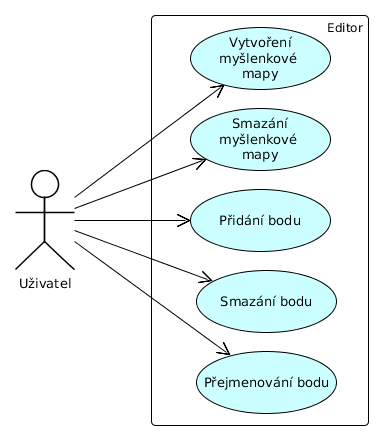
\includegraphics[scale=0.5]{obrazky/use_case}
\par\end{centering}
\caption{Případy užití\label{fig:use_case}}
\end{figure}

Hlavní cíle aplikace jsou:
\begin{itemize}
\item Přidání a odstranění myšlenkové mapy
\item Přidání a odstranění bodu v myšlenkové mapě
\item Přejmenování bodu v myšlenkové mapě
\end{itemize}

%\FloatBarrier

\subsection{Architektura}

Jak je vidět na obrázku \ref{fig:architecture_real}, klienti se budou připojovat přes jeden webový server, který bude mít otevřený port 80. S druhým serverem bude spojený na úrovni Hazelcast clusteru. Vzhledem k situaci, která je blíže popsaná v kapitole \ref{sub:praktCluster}, kdy je webový server připojen do dvou sítí není potřeba šifrování ani nejrůznějších tunelů. Druhý server bude sloužit pro komunikaci s databází a také jako \emph{exporter} myšlenkových map do obrázků ve formátu PNG. Modul \emph{exporter} bude implementován v jazyce Java jako demonstrace polyglot vývoje.

\begin{figure}[h]
\begin{centering}
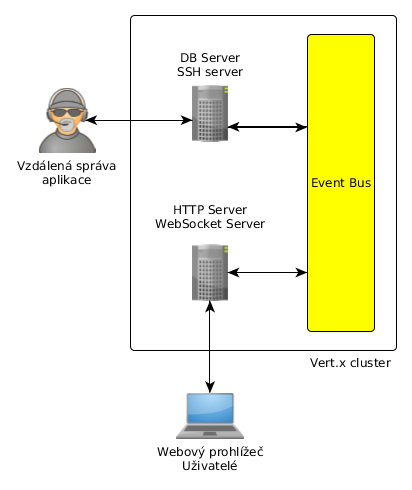
\includegraphics[scale=0.5]{obrazky/architecture_real}
\par\end{centering}
\caption{Architektura nasazené aplikace\label{fig:architecture_real}}
\end{figure}

%\FloatBarrier

\section{Komunikace v reálném čase}\label{sec:realTimeCommunication}

Po načtení myšlenkové mapy přichází na řadu aspekty komunikace v reálném čase. V rámci editoru myšlenkových map budou implementovány tři základní operace.
\begin{itemize}
\item Přidání objektu do myšlenkové mapy
\item Odstranění objektu z myšlenkové mapy
\item Přejmenování objektu v myšlenkové mapě
\end{itemize}

\begin{figure}[h]
\begin{centering}
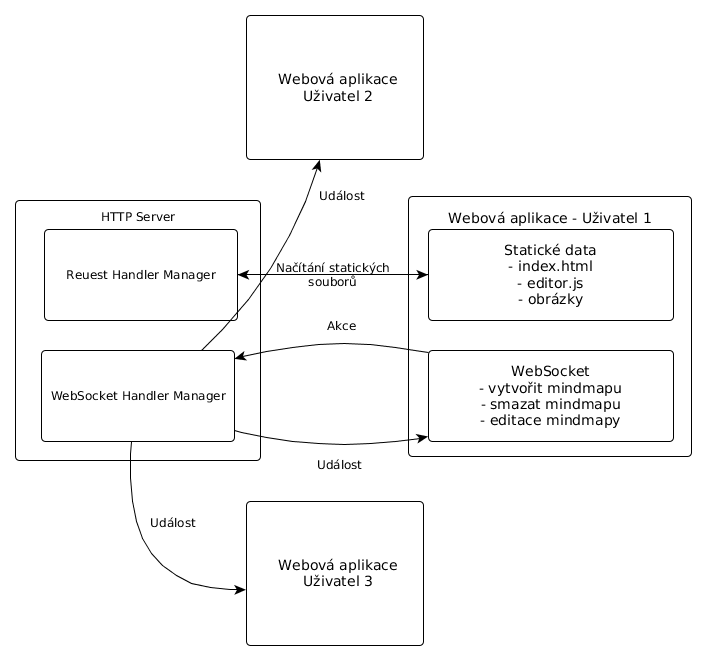
\includegraphics[width	=1\textwidth]{obrazky/realtime_communication}
\par\end{centering}
\caption{Komunikace v reálném čase\label{fig:realtime_communication}}
\end{figure}

V tradiční webové aplikaci by to znamenalo implementaci těchto metod typem požadavek-odpověď jako operací konkrétní API. Při přidání objektu by se zavolala API a nazpět by přišla odpověď, zda-li byla akce úspěšná. Pokud bychom však chtěli mít editor, který by propagoval změny ke všem, kdo mají myšlenkovou mapu otevřenou museli bychom znát přihlášené uživatele, kterým by server poslal notifikaci o změně. Mnohem jednoduší cesta je rozdělení požadavku a odpovědi do dvou částí což odpovídá návrhovému vzoru Command. V takovém případě při otevření webového prohlížeče s danou myšlenkovou mapou dojde k zaregistrování klienta na určitou adresu. V případě jakékoli změny, kterou provede jiný uživatel, dojde k odeslání události všem zaregistrovaným klientům okamžitě v době vykonání události. Tuto situaci lze vidět na obrázku \ref{fig:realtime_communication}. V případě, kdy u uživatele dojde k vyvolání akce, ostatním uživatelům bude zaslána událost, která s sebou nese všechny informace o změně. Všem klientům zaregistrovaným na stejnou adresu přijde stejná událost. Tento typ zasílání zpráv je znám jako návrhový vzor Publish/Subscribe.

\subsection{Akce}

Když bude uživatel chtít změnit myšlenkovou mapu (přidat objekt, odebrat objekt nebo přejmenovat objekt), vyšle akci na server. Tato akce bude poslána přes přemostěný event bus, které jsem představil v kapitole \ref{sub:eventBus}. Na straně serveru je pak verticle, který má zaregistrovány metody na příchozí akce. Samotná akce nemá žádnou návratovou hodnotu, pokud tak dojde k chybě nedojde k vyslání události, která s sebou nese změny myšlenkové mapy.

\subsection{Události}

Pokud uživatel otevře webový prohlížeč s konkrétní myšlenkovou mapou, dojde tak k přihlášení odběru událostí nad touto myšlenkovou mapou. Pokud ji někdo změní, tento uživatel dostane stejnou událost s informací o změně jako každý jiný uživatel přihlášený k odběru událostí.
Na straně klienta tak budou implementovány metody, které budou mít definované chování pro každou z definovaných událostí: přidání, odebrání a přejmenování objektu v myšlenkové mapě.

\section{Vlastní implementace}

Vzhledem k rozsahu práce je v následující kapitole ukázán a popsána většina implementačních částí.

\subsection{Řídící verticle}

Nasazení aplikace na více serverů s sebou přináší malé rozhodnutí. Jestli aplikaci rozdělíme do více menších modulů nebo jednu větší pustíme na více serverech ve více rolích. S přihlédnutím na rozsah aplikace je výhodnější implementovat řídící verticle, který bude mít na starost nasazovat moduly, dle dané konfigurace. Část kódu takového startéru vypadá následovně:

\begin{lstlisting}[caption=Řídící verticle]
var container = require('vertx/container');
var console = require('vertx/console');

var config = container.config;

if("webserver" in config) {
	container.deployModule('io.vertx~mod-web-server~2.0.0-final', config.webserver, config.webserver.workers, function(err, ID){
		if (err) {
			console.log(err)
		}
	});
}
\end{lstlisting}

Každá metoda \emph{deploy} má jako poslední parametr obslužnou rutinu pro případ selhání. V mnoha případech se také hodí ID nasazení, díky němuž lze později toto nasazení zrušit.

Samotný kód vytáhne z třídy \emph{container} konfiguraci celého modulu a zeptá se jestli se v něm nenachází daná role. Potom už jen stačí, aby daný konfigurační soubor obsahoval klíč \emph{webserver} s danou konfigurací, která se nachází níže. Obdobně je implementováno startování editoru, databázového modulu a exportéru. Spuštění modulu či verticle jde samozřejmě i ručně z příkazové řádky.

\begin{lstlisting}[caption=Spuštění modulu z příkazové řádky]
vertx runmod io.majklk~mindmapeditor~0.0.1 -conf /srv/mindmap/conf/webserver.json -instances 3
\end{lstlisting}

Spuštěním modulu z příkazového řádku se Vert.x podívá do deskriptoru modulu, v kterém by měl najít cestu k hlavnímu verticlu. Ten následně spustí a předá mu danou konfiguraci. Samotný verticle pak může pracovat s Vert.x instancí.

\begin{lstlisting}[caption=Konfigurace serveru 1]
{
   "name": "MindMap editor server 1 - HTTP + WebSocket",
    "webserver": {
        "workers": 3,
        "web_root": "web",
        "host": "10.10.10.161",
        "port": 80,
        "bridge": true,
        "inbound_permitted": [
          { "address": "mindMaps.list" },
          { "address": "mindMaps.save" },
          { "address": "mindMaps.delete"},
          { "address": "mindMaps.exporter.svg2png" },
          { "address_re": "mindMaps\\.editor\\..+" }
        ],
        "outbound_permitted": [
          { "address_re": "mindMaps\\.events\\..+" }
        ]
    }
}
\end{lstlisting}

Většina jmen parametrů mluví sami za sebe, kromě \emph{bridge, inbound permitted a outbound permitted}. Pokud je první z nich nastaven na hodnotu \emph{true}, tak začnou platit pravidla, která jsou nadefinována v \emph{inbound permitted, outbound permitted}. Jde o tzv. bridge mezi webovým prohlížečem a Event busem jako takovým. \emph{Inbound permitted} říká jaké adresy se mají pustit dovnitř, analogicky potom \emph{outbound permitted} říká, co může jít ven. Výhodou je pak možnost specifikovat adresu pomocí regulárních výrazů.

\subsubsection{Základní adresářová struktura}

\begin{lstlisting}
main.js //stará se o spouštění celé aplikace v několika rolích
editor.js //obsluha editoru
database.js //obsluha událostí 
web //kořenová složka webové části
\end{lstlisting}

\subsection{Editor}

\begin{lstlisting}[caption=Zaregistrování obslužné rutiny v jazyce JavaScript]
var eb = vertx.eventBus;

var mujHandler = function(zprava) {
  console.log('Přišla zpráva ' + zprava);
}

eb.registerHandler('test.tisk', mujHandler);
\end{lstlisting}

Obdobně to pak vypadá v ostatních jazycích. 

\begin{lstlisting}[caption=Zaregistrování obslužné rutiny v jazyce Java]
EventBus eb = vertx.eventBus();

Handler<Message> mujHandler = new Handler<Message>() {
    public void handle(Message zprava) {
        System.out.println("Přišla zpráva " + zprava.body);
    }
};

eb.registerHandler("test.tisk", mujHandler);
\end{lstlisting}

Na podobném principu je pak postaven zbytek serverové části. Na jednotlivé události jsou zaregistrovány podobné obslužné rutiny, které většinou dohledají konkrétní mapu a provedou nad ní nějakou změnu. Výslednou mapu uloží a pošlou událost všem klientům jako je vidět na diagramu \ref{fig:realtime_communication}.

\begin{lstlisting}[caption=Publikování zprávy v jazyce JavaScript]
eventBus.publish('editor.udalosti.'+mindMap._id, {"udalost": "bodPridan", parentKey: args.parentKey, node: newNode})
\end{lstlisting}

Díky metodě \emph{publish}, která je samozřejmě dostupná ve všech jazycích můžeme publikovat událost všem klientům, kteří mají zaregistrovanou obslužnou rutinu na identickou adresu, která je unikátní pro každou mapu.

\vspace{0.5cm} % fix

\subsection{Integrace s databází MongoDB}

Vzhledem k jednoduchosti aplikace nebyl vytvořen diagram tříd. V aplikaci budou pouze dva modely, a to mapa a její potomek, který se od mapy liší pouze tím, že má místo globálního unikátního identifikátoru pouze unikátní identifikátor v rámci jedné mapy.

V centrálním repozitáři již existuje modul pro komunikaci s MongoDB\footnote{https://github.com/vert-x/mod-mongo-persistor}, který poskytuje jednoduchou API pro asynchronní komunikaci s databází. Zaregistrujeme tedy obslužnou rutinu pro uložení myšlenkové mapy. Obdobně pak pro každou akci z definovaných cílů.

\begin{lstlisting}[caption=Uložení myšlenkové mapy do databáze]
var eventBus = require('vertx/event_bus');
var console = require('vertx/console');

eventBus.registerHandler('mindMaps.save', function(mindMap) {
	dotaz_do_databaze = {action: "save", collection: "mindMaps", document: mindMap}
	eventBus.send('vertx.mongopersistor', dotaz_do_databaze, function(reply) {
		if (reply.status === "ok") {
			// vše v pořádku
		} else {
			console.log(reply.message);
		}
	});
});

\end{lstlisting}

\begin{lstlisting}[caption={Konfigurace serveru 2},label=confServ2]
{
    "name": "MindMap editor server 2 databázový modul, obrazkový exporter",
    "exporter": {
        "workers": 5
    },
    "mongodb": {
        "address": "vertx.mongopersistor",
        "host": "localhost",
        "port": 27017,
        "db_name": "mindmap_editor",
        "pool_size": 20
    },
    "shell": {
      "crash.auth": "simple",
      "crash.auth.simple.username": "admin",
      "crash.auth.simple.password": "heslo",
      "crash.ssh.port": 2000
    }
}
\end{lstlisting}

\begin{description}
\item[\_id] unikátní identifikátor\footnote{podtržítkem se běžně označující neměnné proměnné}
\item[name] název samotné mapy
\item[children] potomci
\end{description}

\begin{lstlisting}
\end{lstlisting}

\begin{lstlisting}
{
	"_id": "1234-6545-5612-3456",
	"name": "Živočichové",
	"children": [
		{
			"key": "1",
			"name": "Obratolvci",
			"children": [
				{
					"key": "2",
					"name": "Ryby"
				},
				{
					"key": "3",
					"name": "Plazi"
				}
			]
		},
		{
			"key": "4",
			"name": "Bezobratlí"
		}
	]
}
\end{lstlisting}

\subsubsection{Struktura webové části}

\begin{lstlisting}
index.html
js/client.js //obsluha editoru
js/editor.js //vykreslování grafu - D3.js
js/vertxbus.js //knihovna pro napojení na Event Bus
css //složka pro kaskádové styly
\end{lstlisting}


\subsubsection{Event Bus v prohlížeči}

Nejdůležitější částí klientské aplikace je Vert.x vrstva nad SockJS\cite{sockjs}, která zabaluje komunikaci se serverem na protokolu WebSocket\cite{webSockets}. Knihovna naváže a udržuje neustálé spojení se serverem. Implementací metod \emph{eb.onopen a eb.onclose} může patřičně reagovat na otevření a uzavření spojení. Jediným parametrem samotného EventBusu je pak URL adresa na kterou se má připojit.

\begin{lstlisting}[caption=Připojení Event busu z prohlížeče a inicializace editoru]
var eb = new vertx.EventBus(window.location.protocol + '//' + window.location.hostname + ':' + window.location.port + '/eventbus');

eb.onopen = function() {
	//tato metoda se volá po úspěšném navázání komunikace
	//zde již můžeme posílat zprávy
	eb.send("mindMaps.save", mapa, function(reply){
		eb.send("mindMaps.find", mapa._id, function(mindMap){
			new MindMapEditor(mindMap, eb); //inicializace editoru
		});	
	});
}
\end{lstlisting}

\subsubsection{D3.js}

Vynikající knihovnou pro práci s grafy je D3.js, napsaná v jazyce JavaScript. Díky stovkám již hotových ukázek si stačí jen vybrat, kterou použít. Všechny jsou totiž volně dostupné. Pro vykreslení myšlenkových map tak poslouží Collapsible Tree\cite{d3js}, který se výborně hodí právě pro stromové struktury. Implementace webového editoru je v souboru \emph{editor.js}

\begin{lstlisting}[caption=D3.js nicializace dat]
var tree = d3.layout.tree()
		    .size([vyska, sirka]);

var diagonal = d3.svg.diagonal()
		   .projection(function(d) { return [d.y, d.x]; });
		   
d3.json(mindMap);
\end{lstlisting}


\section{Polyglot vývoj a moduly}\label{sec:praktickyModuly}

Pro větší znovupoužitelnost je vhodné své aplikace balit do modulů, které pak lze snadno distribuovat v různých formátech. Aby se z editoru stal modul, musí být adresářová struktura upravena následovně.

\begin{lstlisting}
mods //složka pro další moduly
lib //složka pro ostatní knihovny např. další jar soubory
main.js //stará se o spouštění celé aplikace v několika rolích
editor.js //obsluha editoru
database.js //obsluha událostí 
web //kořenová složka webové části
mod.json //deskriptor modulu
\end{lstlisting}

Classloader při startu modulu automaticky načte všechny knihovny nacházející se ve složce \emph{lib}. Ručně to lze pak přes parametr \emph{-cp}\footnote{ClassPath}. Aby byl modul spustitelný, musí deskriptor modulu obsahovat parametr \emph{main}. Což je cesta a jméno hlavního verticle. Modul, který nemá specifikovaný parametr \emph{main} lze pak snadno použít v jiném modulu pomocí parametru \emph{includes}. Modul se pak musí nacházet ve složce \emph{mods}. Nastavením parametru \emph{worker} na \emph{true} docílíme vyčlenění všech verticlů z asociace na Event loop jak bylo řečeno v \ref{sub:hybrid}. Parametr \emph{auto-redeploy} se hodí především v časech vývoje, při každé změně kódu dojdu k novému nasazení modulu. 
\begin{lstlisting}
{
  "main": "main.js",
  "worker": true,
  "includes": "io.majklk~mindmapeditor~0.0.1",
  "auto-redeploy": true
}
\end{lstlisting}

Jmenná konvence modulů vychází ze Java konvence\cite{javaPKG} pro pojmenování balíčků kterou rozšiřuje o číslo verze \emph{com.mycompany~my-mod~1.0}.
Pro publikování modulu jsou pak důležité nejrůznější metadata, které je dobré specifikovat.
\begin{lstlisting}[caption=Deskriptor modulu]
{
	"developers": ["Michael Kutý"],
	"name": "MindMap Editor",
	"version": "0.0.1",
	"description": "Jednoduchý editor myšlenkových map",
	"keywords": ["vert.x,mongodb,d3js"]
}  
\end{lstlisting}

\begin{lstlisting}[caption=Spuštění modulu v jazyce Java]
container.deployModule("io.majklk~mindmapeditor~0.0.1", JSONconfig);
\end{lstlisting}

\begin{lstlisting}[caption=Verticle v jazyce Java]

import org.vertx.java.core.Handler;
import org.vertx.java.core.eventbus.Message;
import org.vertx.java.core.json.JsonObject;
import org.vertx.java.platform.Verticle;

//třída musí rozšiřovat třídu Verticle
public class ImageExporter extends Verticle {
	
	public void start() {
		Handler<Message<JsonObject>> exportHandler = new Handler<Message<JsonObject>>() {
			public void handle(Message<JsonObject> message) {
				String svg = message.body().getString("svg");
				String css = message.body().getString("css");
				//odpověď volajícímu req/res
				message.reply(new JsonObject().putString("data", getPng(svg, css)));
			}
		};
		//zaregistrování obslužné rutiny
		vertx.eventBus().registerHandler("mindMaps.exporter.svg2png", exportHandler);
	}

	private String getPng(String svg, String css) { 
		\\tělo metody
	}
}
\end{lstlisting}

\begin{figure}
\begin{centering}
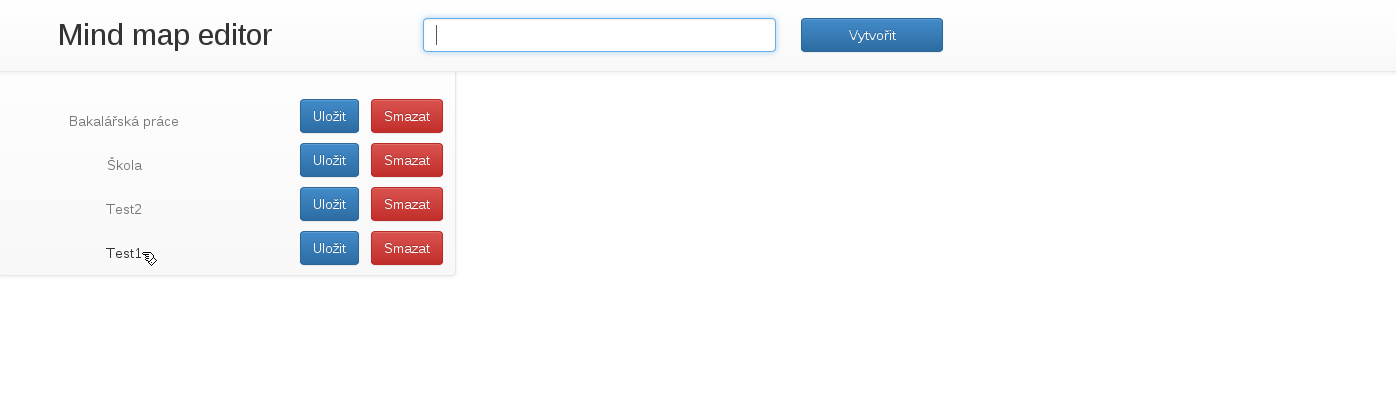
\includegraphics[width	=1\textwidth]{obrazky/mindmap1}
\par\end{centering}
\caption{Webová aplikace\label{fig:midnmap1}}
\end{figure}

\begin{figure}
\begin{centering}
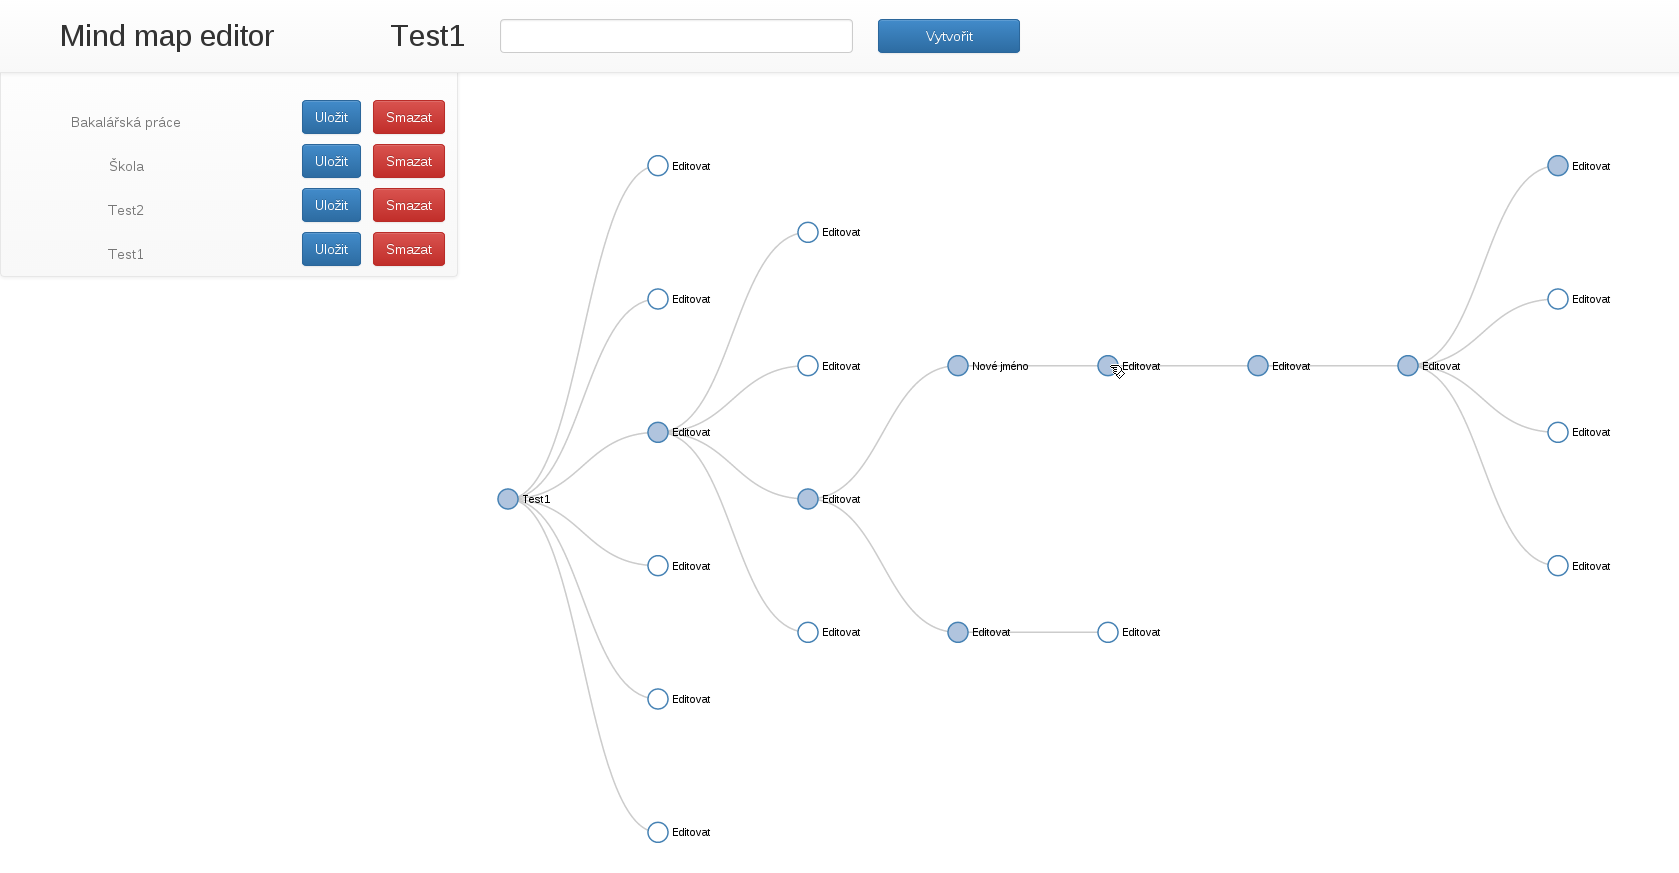
\includegraphics[width	=1\textwidth]{obrazky/mindmap2}
\par\end{centering}
\caption{Webová aplikace - otevření myšlenkové mapy\label{fig:midnmap2}}
\end{figure}

\begin{figure}
\begin{centering}
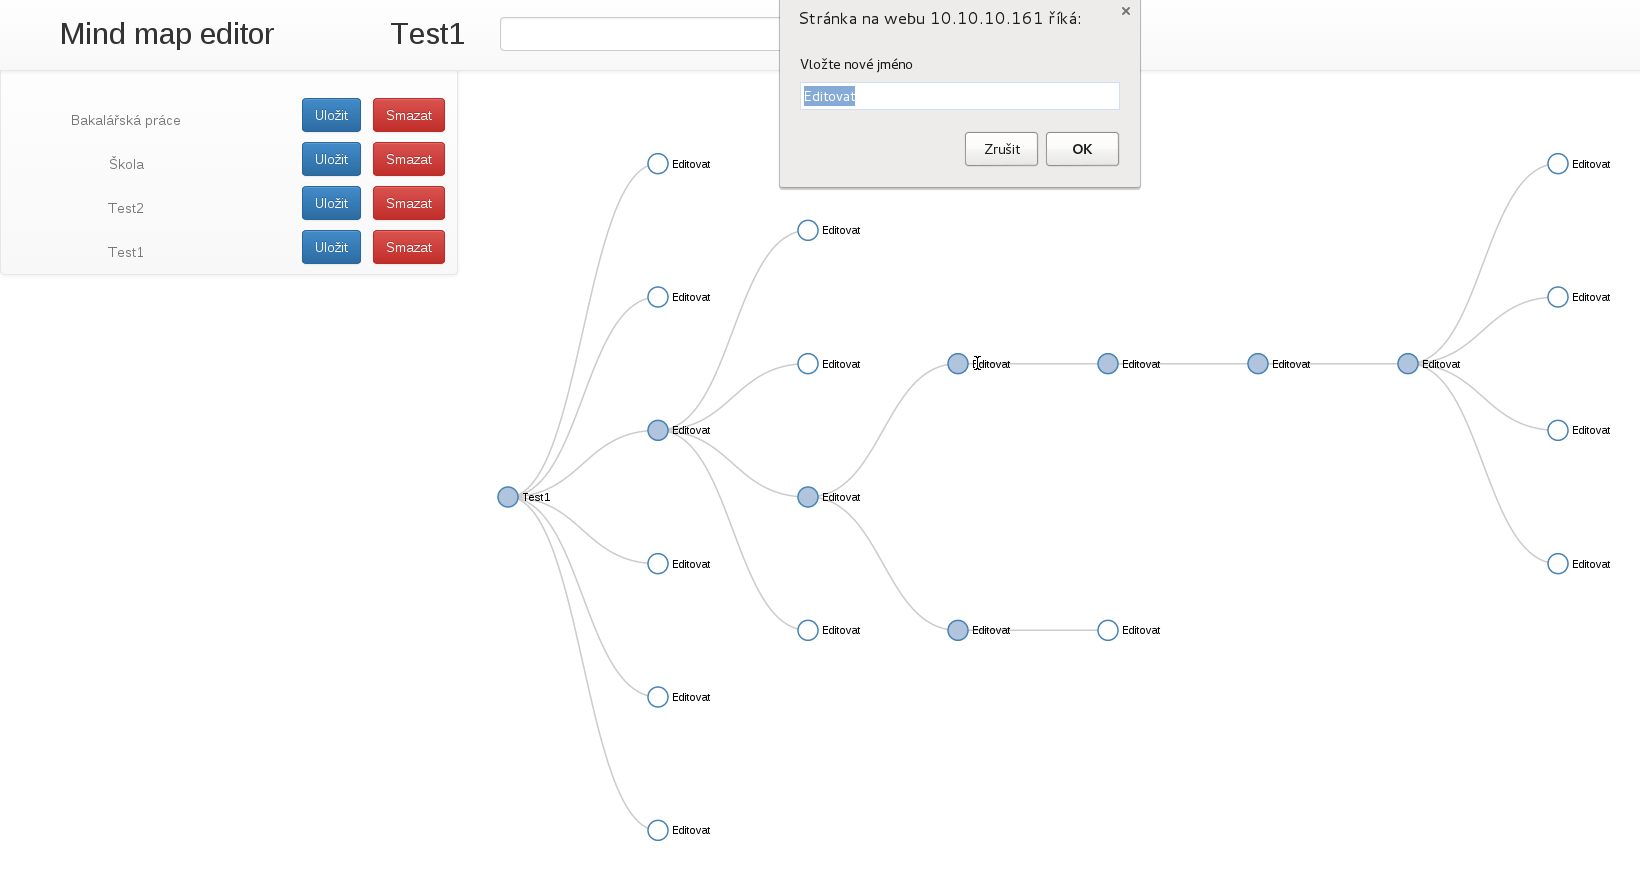
\includegraphics[width	=1\textwidth]{obrazky/mindmap3}
\par\end{centering}
\caption{Webová aplikace - akce - editace\label{fig:midnmap3}}
\end{figure}

\section{Základní software}

Jádrem serveru je operační systém Ubuntu\cite{ubuntu} 14.04 LTS\footnote{dlouhodobá podpora} Server Edition s kódovým označením 
Trusty Tahr. Je to osvědčený systém, který bude má zaručenou podporu do roku 2019. Systém má aplikaci pro správu softwarových balíků 
aptitude. Všechny aplikace kromě samotného Vert.x jdou hravě nainstalovat pře tento systém.

\subsection{Java}

Jako hlavní přísadou celého prostředí je otevřená implementace Java Platform, knihovna OpenJDK ve verzi 7.

\subsection{Vert.x}

Jediná služba, která se zatím nenachází jako systémový balíček je samotný Vert.x. Pro jeho instalaci je nutné stáhnout distribuci ze stránek platformy. Tento archiv potom rozbalit do požadované lokace. Následně stačí v závislosti na konkrétním systému přidat soubor \emph{vertx/bin/vertx} do systémové proměnné \emph{PATH}. Poté by měla být funkční interakce s platformou pomocí příkazové řádky. Příklad proměnné \emph{PATH} lze vidět v kapitole \ref{sub:service}. Správné nastavení lze otestovat napsáním \emph{vertx} do příkazové řádky. Správný výstup jsou pak pomocné informace pro komunikaci s platformou tzv. help.

\subsection{Databázový server}

Pro ukládání myšlenkových map je použita NoSQl databáze MongoDB ve verzi 2.6. MongoDB má za sebou více než pět let vývoje a několik obřích investic\cite{mongodb} do dalšího vývoje. V dnešní době existuje nespočet NoSQL databází, vzhledem k tomu, že již existuje Vert.x modul pro pohodlnou asynchronní spolupráci s touto databází, byla vybrána pravě tato NoSQL databáze. Pro instalaci stačí využít balíčkovací systém aptitude. Nastavení databáze lze ponechat ve výchozím stavu, kdy databáze naslouchá na portu 27017. Což lze vidět i z konfigurace aplikace v ukázce kódu \ref{confServ2}.

\begin{lstlisting}
apt-get install mongodb-server -y
\end{lstlisting}

\subsection{Nasazení produkční služby}\label{sub:service}

V současné verzi, (2.1.2) Vert.x nepodporuje běh v režimu daemon\footnote{je program, který běží v pozadí, čeká na události, které nastanou, reaguje na ně a poskytuje služby.}. Nasazení v režimu daemon je však nutnost pro běh v produkčním prostředí. Pro běh aplikace MindMap editoru byla využita systémová služba Supervisord\footnote{supervisord.org}, která běží jako linuxový daemon a stará se o běh aplikace, v případě pádu se ji pokusí znovu nasadit. Samotná konfigurace služby pro běh v Supervisordu pak obsahuje základní parametry. Ve verzi 3.0 je však plánovaná funkce běhu v režimu daemona a nebude tak tato berlička potřeba.

\begin{lstlisting}[caption=Konfigurace produkční služby]
[program:vertx_mindmap_editor]
directory=/srv/mindmap/app
environment=PATH="/srv/vert.x-2.1RC3/bin/vertx"
environment=JAVA_HOME="/usr/lib/jvm/java-7-openjdk-amd64/"
command=vertx runmod io.majklk~mindmapeditor~0.0.1 -conf /srv/mindmap/conf/allinone.json
user=root
autostart=true
autorestart=true
redirect_stderr=true
stdout_logfile=/srv/mindmap/app/app.log
stderr_logfile=/srv/mindmap/app/error.log
startsecs=10
stopwaitsecs=600
\end{lstlisting}

Nejdůležitější parametry jsou \emph{environment} a \emph{command}, které umožňují pohodlně spustit libovolnou aplikaci jako daemona.

\subsection{Interakce s Vert.x}\label{sub:interaction}

Díky modulu CrasHub Shell\footnote{https://github.com/crashub/mod-shell} se lze protokolem SSH\footnote{Secure Shell} přihlásit přímo do Vert.x. Modul pak nabízí možnost interakce s jednotlivými komponentami samotného Vert.x. Lze například posílat zprávy přes Event Bus nebo nasazovat nové moduly za běhu celé aplikace.
\begin{figure}[h]
\begin{centering}
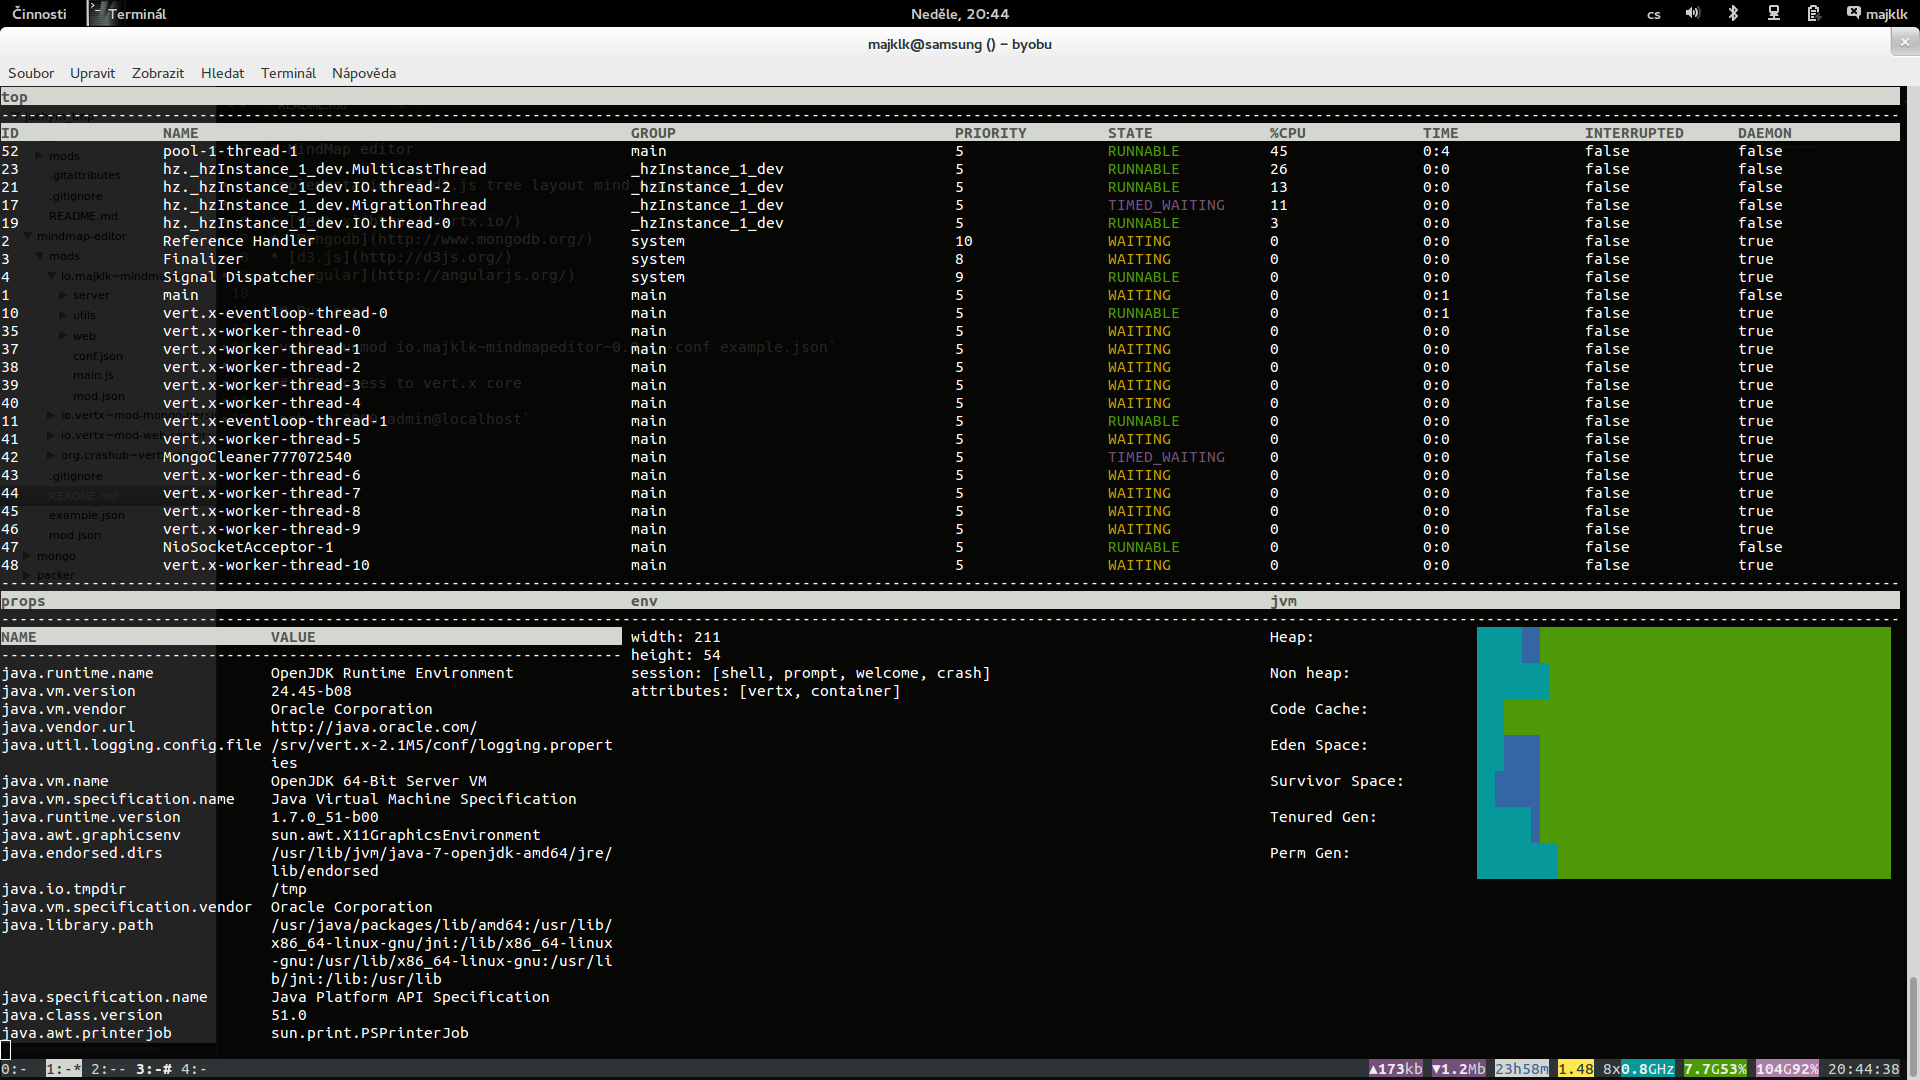
\includegraphics[scale=0.21]{obrazky/real_interaction}
\par\end{centering}
\caption{Modul CrasHub Shell\label{fig:real_interaction}}
\end{figure}

Pro nasazení modulu stačí přidání klíče \emph{shell} do konfigurace server 2. Po nasazení aplikace začne tento server poslouchat na portu 2000.

\begin{lstlisting}[caption={Konfigurace modulu CrasHub Shell},label=confServ2]
{
    "name": "MindMap editor server 2 databázový modul, obrazkový exporter",
    "shell": {
      "crash.auth": "simple",
      "crash.auth.simple.username": "admin",
      "crash.auth.simple.password": "heslo",
      "crash.ssh.port": 2000
    }
}
\end{lstlisting}

Samotný modul nabízí nepřeberné množství možností jak spravovat aplikace nebo ji naživo škálovat. Lze také jednoduše přidat vlastní příkazy a rozšířit tak možnosti tohoto modulu. Na obrázku \ref{fig:real_interaction} je hlavní přehledová stránka, na které lze vidět činnost vytížení a status všech vláken v celém clusteru. Dostupné jsou také informace o velikosti zásobníku, paměti či verze Javy. 

\section{Škálování}\label{sub:Scaling}

Škálování je nedílnou součástí životního cyklu aplikace. Ne zřídka dojde aplikace do situace, kdy začne být pomalá či často padat pod velkým náporem klientů. V následující kapitole proto rozebírám možnosti škálování Vert.x aplikací.

\FloatBarrier

\subsection{Vertikální}

Samotné vertikální škálování lze efektivně řešit až na aplikační úrovni. Jak již bylo zmíněno v kapitole \ref{sub:multireactor} voláním \emph{Runtime.getRuntime().availableProcessors()}, lze získat počet procesorových jader a s tím dále pracovat. Upravením předchozích příkazů však docílíme shodného výsledku.

\begin{lstlisting}
command=vertx runmod io.majklk~mindmapeditor~0.0.1 -instances 4 -conf
\end{lstlisting}

\subsection{Horizontální}\label{sub:praktCluster}

Dle návrhu architektury na obrázku \ref{fig:architecture_real} bude aplikace nasazena na dva servery. První bude naslouchat na port 80 a poběží zde Webový server(HTTP Server). Tento server má vnitřní IP adresu \emph{10.10.10.161}. Druhé rozhraní má připojené do internetu. Na druhém serveru je část aplikace, která komunikuje s databází a modul pro vzdálenou interakci s Vert.x. Jeho IP adresa je \emph{10.10.10.162}. Pro propojení obou instancí je potřeba upravit spouštěcí příkaz v konfiguraci Supervisoru.

\begin{lstlisting}[caption=Spuštění clusteru na Serveru 1]
command=vertx runmod io.majklk~mindmapeditor~0.0.1 -conf /srv/mindmap/conf/webserver.json -cluster -cluster-host 10.10.10.161
\end{lstlisting}

\begin{lstlisting}[caption=Spuštění clusteru na Serveru 2]
command=vertx runmod io.majklk~mindmapeditor~0.0.1 -conf /srv/mindmap/conf/dbserver.json -cluster -cluster-host 10.10.10.162
\end{lstlisting}

\subsection{Ladění výkonnosti}\label{sub:performenceScale}

Hlavní sada vláken, tedy event loopů je ve výchozím nastavení na hodnotě odpovídající volání funkce \emph{Runtime.getRuntime().availableProcessors()}. Tuto hodnotu lze změnit nastavením systémové proměnné \emph{vertx.pool.eventloop.size}. Nastavením \emph{vertx.pool.worker.size} pak lze změnit velikost poolu pro dlouhotrvající operace, která je ve výchozím nastavení na hodnotě 20.

\section{Vysoká dostupnost}

Pro zajištění vysoké dostupnosti klíčových prvků aplikace, je potřeba upravit architekturu clusteru. Před webový server je postaven load balancer\footnote{služba zajištující vyrovnávání zatížení} v tomto případě HA proxy, která při úpadku jednoho z webových serverů přesměruje komunikaci na server druhý. Vert.x cluster je rozdělený na dvě HA skupiny (obr.\ref{fig:architecture_ideal}), které se liší svým zaměřením. První dva servery slouží jako webové a jsou napojeny na HA proxy. Další dva slouží pro komunikaci s databází, která na nich, přímo běžet nemusí. V této HA skupině je dále modul pro interakci s Vert.x. Díky specifikaci HA skupiny nikdy nedojde k nasazení modulu na webovém serveru a tedy otevření SSH na portu 2000.

\begin{lstlisting}[caption=Vysoká dostupnost na databázovém serveru 2]
command=vertx runmod io.majklk~mindmapeditor~0.0.1 -conf /srv/mindmap/conf/dbserver.json -cluster-host 10.10.10.162 -ha -hagroup skupina-1
\end{lstlisting}

Když je specifikován parametr \emph{-ha}, lze automaticky vypustit parametr \emph{-cluster}.

\begin{figure}
\begin{centering}
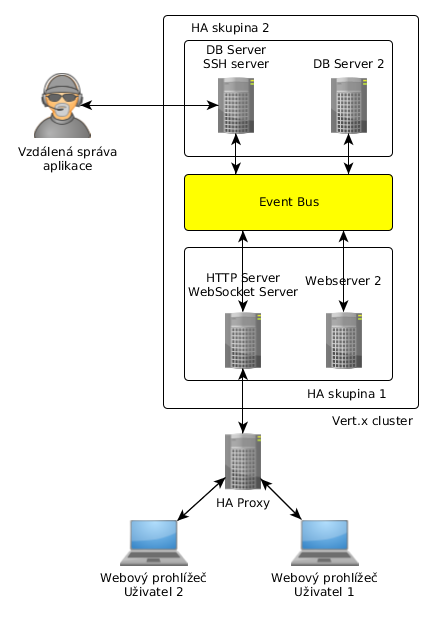
\includegraphics[scale=0.5]{obrazky/architecture_ideal}
\par\end{centering}
\caption{Ideální architekutra nasazení aplikace\label{fig:architecture_ideal}}
\end{figure}

\section{Integrace do stávájící Java aplikace}

Pokud je to jakkoliv jen možné, je vhodné se integraci vyhnout. Pokud však nejde jinak, existují dvě varianty jak integrovat platformu:

\begin{enumerate}
\item PlatformManager
\item Pomocí jar souboru
\end{enumerate}

\begin{lstlisting}[caption=Integrace do stávající Java aplikace]

//díky platform managerovi lze provádět stejné úkony jako v příkazové řádce
PlatformManager pm = null;
pm = PlatformLocator.factory.createPlatformManager();

JsonObject conf = new JsonObject().putString("foo", "wibble");

pm.deployModule("com.mycompany~my-module~1.0", conf, 10, new AsyncResultHandler<String>() {
    public void handle(AsyncResult<String> asyncResult) {
        if (asyncResult.succeeded()) {
            System.out.println("Deployment ID is " + asyncResult.result());
        } else {
            asyncResult.cause().printStackTrace();
        }
    }
});
\end{lstlisting}

V takovém případě bude platforma hledat \emph{cluster.xml} a \emph{repos.txt} v proměnné classpath.